\section{Détails des mèmes}
\label{sec:fullmemes}
\subsection{Dufu is very busy}


\zh{杜甫很忙}

Le poète chinois Du Fu de la dynastie Tang a également connu un retour fulgurant sous la forme de peintures détournées le mettant en scène dans des situations improbables : ``Du Fu est vraiment très occupé'' \zh{杜甫很忙}. 


Voir aussi :
\url{http://knowyourmeme.com/memes/du-fu-is-busy}
et
\url{http://wenku.baidu.com/view/941e25c805087632311212aa.html}

\begin{figure}[ht]
    \centering
    \subfloat[]{
\includegraphics[scale=.4]{figures/annexes/dufu/8c7.jpg}}
    \subfloat[]{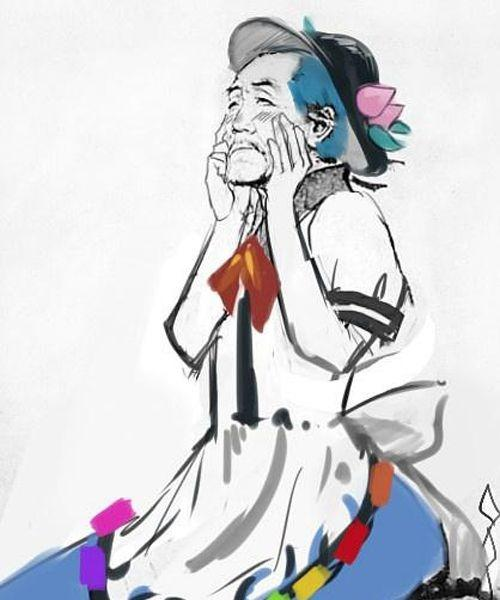
\includegraphics[scale=.3]{figures/annexes/dufu/8dd.jpg}}
    \subfloat[]{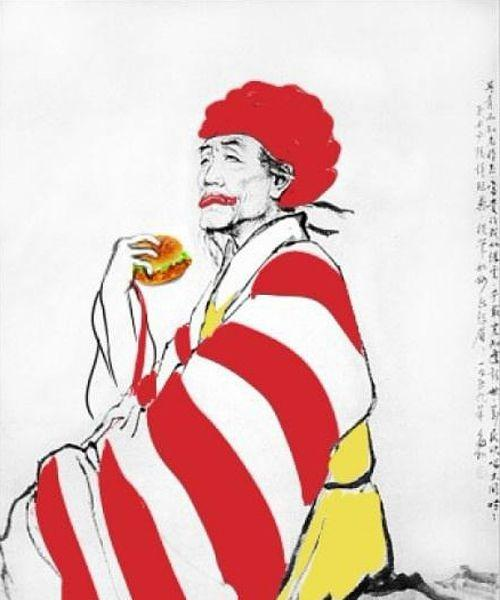
\includegraphics[scale=.3]{figures/annexes/dufu/b5f.jpg}}
    \newline
    \subfloat[]{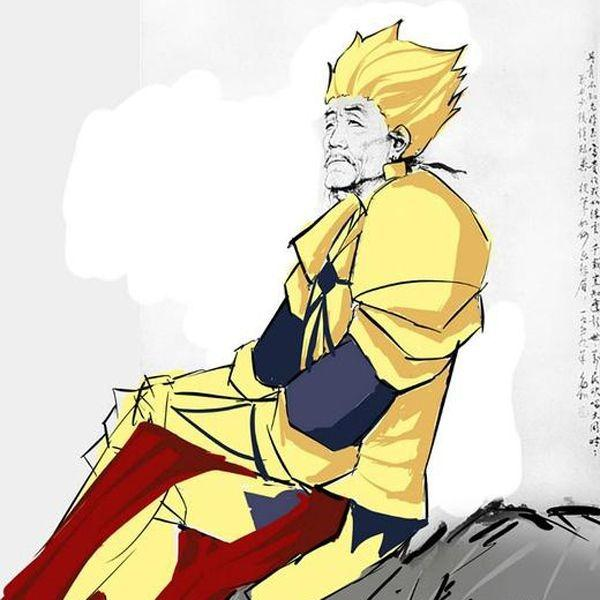
\includegraphics[scale=.3]{figures/annexes/dufu/bb3.jpg}}
    \subfloat[]{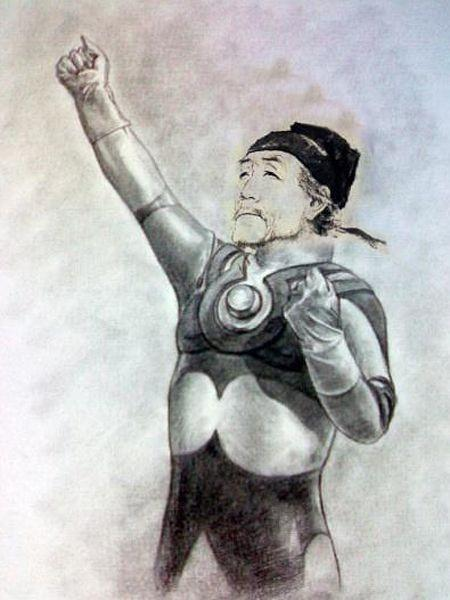
\includegraphics[scale=.3]{figures/annexes/dufu/bd8.jpg}}
    \subfloat[]{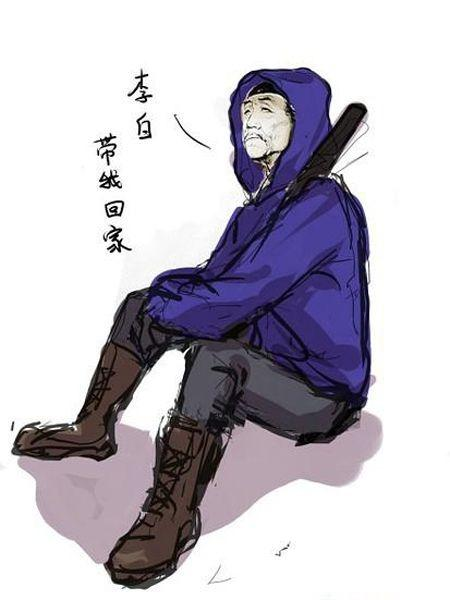
\includegraphics[scale=.3]{figures/annexes/dufu/d09.jpg}}
    \caption{
      Dufu is very busy 
    }
\end{figure}

\clearpage

\subsection{Yuan Fang, qu'en penses tu?}

Une série policière très prisée présentant un couple de détectives enquêtant dans la Chine médiévale procura notamment de bonne doses de rire aux spectateurs. Dialogue récurrent de la série, la phrase ``Yuanfang, qu'en penses-tu'' (\zh{元芳,你怎么看?}) s'est hissé en peu de temps à une célébrité semblable au \textit{``élémentaire''} de Sherlock Holmes au Dr. Watson. 

\begin{figure}[ht]
    \centering
    \subfloat[]{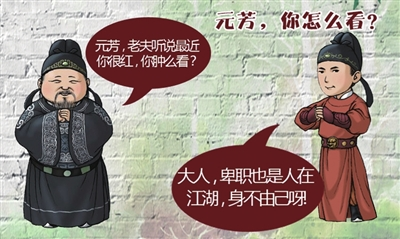
\includegraphics[scale=.4]{figures/annexes/yuanfang/50fa21e4d4994.jpg}}
    \subfloat[]{
\includegraphics[scale=.6]{figures/annexes/yuanfang/960a304e251f95ca67b3a568c9177f3e660952ad.jpg}}
    \newline
    \subfloat[]{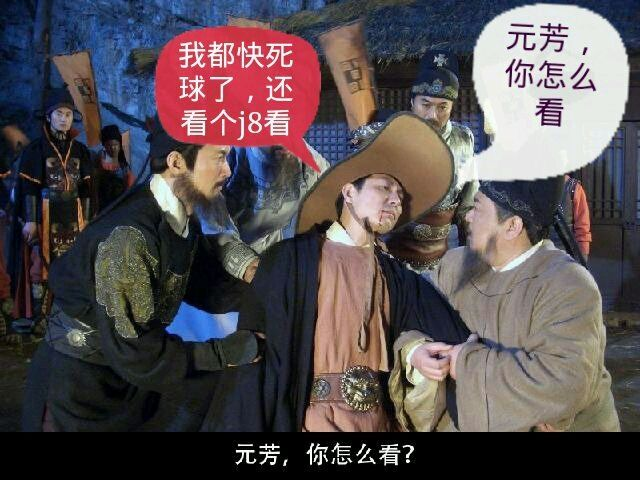
\includegraphics[scale=.3]{figures/annexes/yuanfang/2012102210340971752.jpg}}
    \subfloat[]{
\includegraphics[scale=.3]{figures/annexes/yuanfang/d4f21080968f3187.png}}
    \newline
    \subfloat[]{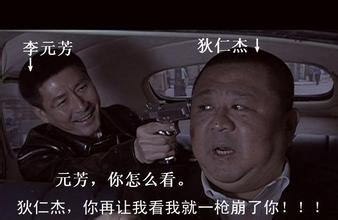
\includegraphics[scale=.5]{figures/annexes/yuanfang/u=4077910649,4163896412&fm=21&gp=0.jpg}}
    \subfloat[]{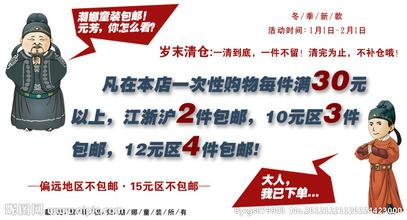
\includegraphics[scale=.5]{figures/annexes/yuanfang/ad.jpg}}
    \caption{
      Exemples d'images du mème \textit{Yuanfang}
    }
\end{figure}

\clearpage

\subsection{Biaoge}
\label{sec:biaoge}

En Août 2012, Yang Dacai, directeur du Bureau de Supervision de la Sécurité Routière de la province du Shanxi, se rend sur les lieux d'un accident de bus ayant fait 36 morts. Une photo diffusée sur Internet le montre discutant avec un policier, arborant un grand sourire. Agacé par cette excès d'incivilité, les internautes commencent à faire des recherches à son sujet et se rendent compte que l'officiel chinois arborent à chaque apparition une montre différente, toutes de marques prestigieuses. Les internautes le renomme rapidement \textit{le frère aux montres} (\textit{biaoge}) et collectent les photos de ses différentes montres de luxe comme autant de preuves manifestes de sa corruption. Quelques jours plus tard, Yang Dacai est démis de ces fonctions. Il sera par la suite jugé et condamné pour corruption, assorti d'une peine de 12 ans de prison. 

\begin{figure}[h!]
    \centering
    \subfloat[]{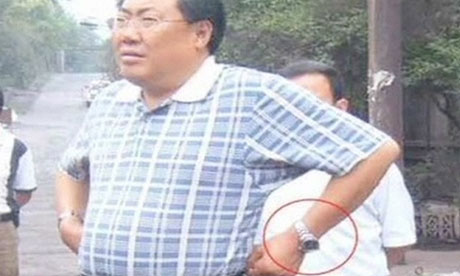
\includegraphics[scale=.4]{figures/annexes/biaoge/Yang-Dacai-wearing-one-of-010.jpg}}
    \subfloat[]{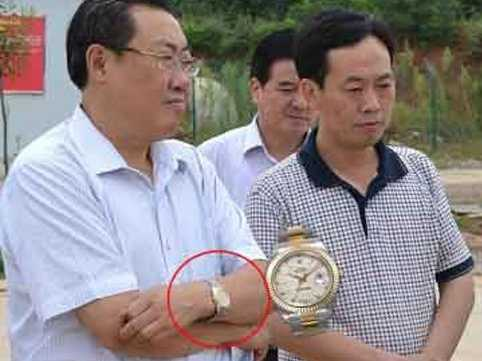
\includegraphics[scale=.3]{figures/annexes/biaoge/chinese-official-photographed-smirking-after-a-traffic-accident-that-left-36-dead-has-been-fired.jpg}}
    \newline
    \subfloat[]{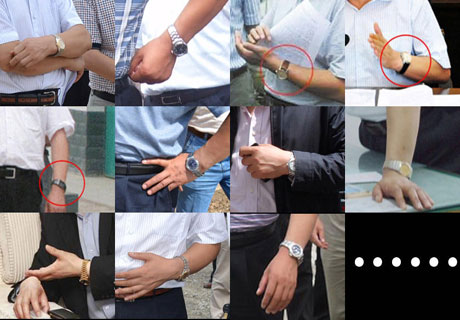
\includegraphics[scale=.3]{figures/annexes/biaoge/201209120198.jpg}}
    \subfloat[]{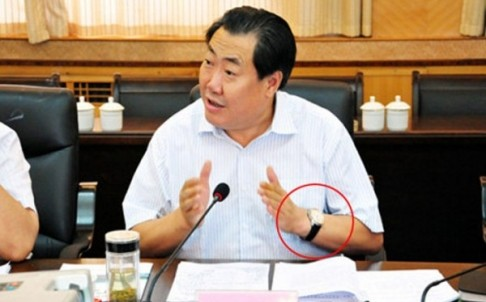
\includegraphics[scale=.3]{figures/annexes/biaoge/yang-dacai.jpg}}
    \caption{
      Images du mème entourant les montres de Yang Dacai
    }
\end{figure}

\clearpage
\subsection{Sex Tape}
\label{sec:sextape}

La vidéo diffusée montrant Lei Zhengfu, le secrétaire du Parti dans le district de Beibei à Chongqing dans le plus simple appareil en compagnie d'une de ses maîtresses (\textit{sextape}). A peine 63h après la publication de cette vidéo avec le titre ``Lei, the secretary who accepts sex bribes'', Lei fut mis à pied de ses fonctions politiques. Cette vidéo qui avait été tournée 4 ans auparavant été utilisée depuis plusieurs années par un promoteur immobilier de la ville de Chongqing pour faire chanter Lei Zhengfu. 

Voir aussi :
\url{http://en.wikipedia.org/wiki/Lei_Zhengfu}
et 
\url{http://www.viddler.com/v/41bf67b2}, consulté le 7 Juillet à 12:32

\begin{figure}[h!]
    \centering
    \hfill
    \subfloat[Image tirée de la vidéo]{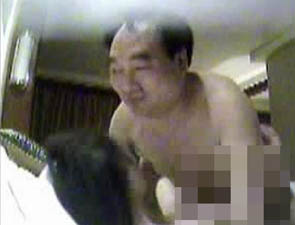
\includegraphics[scale=.8]{figures/annexes/sextape/Lei-Zhengfu.jpg}}
    \hfill
    \subfloat[Photo de la femme]{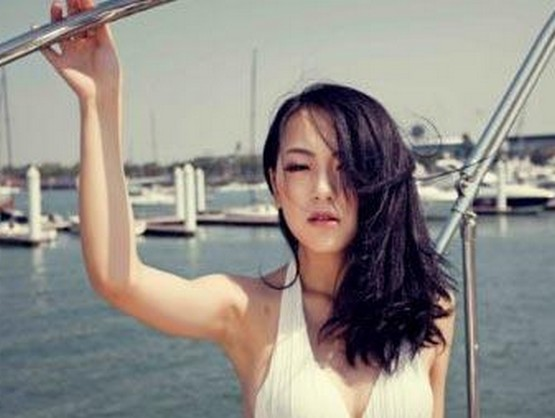
\includegraphics[scale=.3]{figures/annexes/sextape/Lei-Zhengfu-Tape-Scandal-Leads-To-Chinese-Officials-Firing7.jpg}}
    \hfill
    \newline
    \hfill
    \subfloat[Détournement d'un internaute]{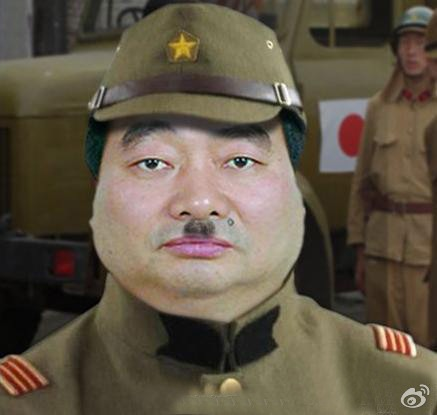
\includegraphics[scale=.5]{figures/annexes/sextape/lei05.jpg}}
    \hfill
    \subfloat[Détournement d'un internaute]{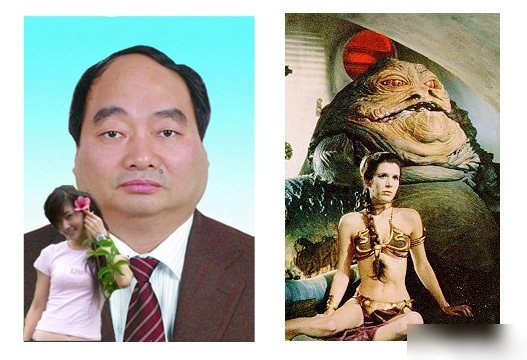
\includegraphics[scale=1.3]{figures/annexes/sextape/LeiJabba.jpg}}
    \hfill
    \caption{
      Exemples d'image du mème concernant la sextape de Lei Zhengfu. Images d'après l'article ``Sex tape official stands trial in Chongqing'' dans le \textit{People's Daily}, \url{http://english.peopledaily.com.cn/90882/8290628.html} et \url{http://www.dailymail.co.uk/news/article-2239300/Zhao-Hongxia-Teenage-honeytrap-brought-Chinese-Communist-Party-official-sex-tape-pictures-leaked-online.html} consulté le 7 Juillet à 12:32
    }
\end{figure}





\clearpage
\subsection{Qiegao}

http://world.time.com/2012/12/05/dont-let-them-eat-cake-how-ethnic-tensions-in-china-explode-on-the-streets/


\begin{figure}[h!]
    \centering
    \subfloat[Un vendeur de qiegao]{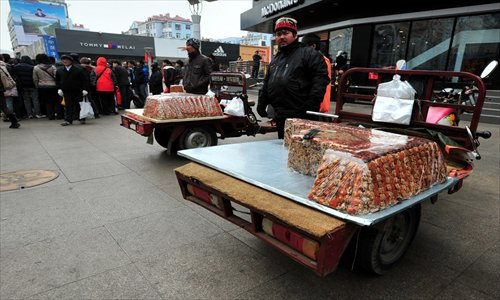
\includegraphics[scale=.65]{figures/annexes/qiegao/91914349-4fce-4373-b7dc-9fe05a0a28bf.jpeg}}
    \subfloat[Le gâteau]{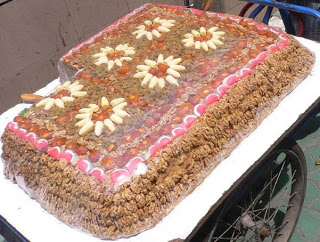
\includegraphics[scale=.7]{figures/annexes/qiegao/Qie-Gao.jpeg}}
    \newline
    \subfloat[Une image de l'affrontement avec la police posté par un utilisateur de Sina Weibo]{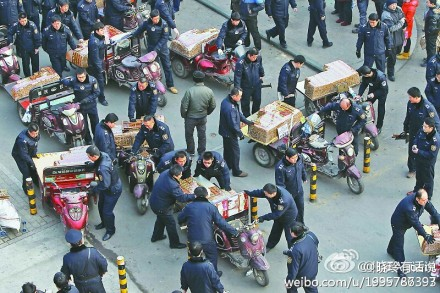
\includegraphics[scale=.65]{figures/annexes/qiegao/1.jpg}}
    \subfloat[Création d'un internaute montrant combien le qiegao est cher]{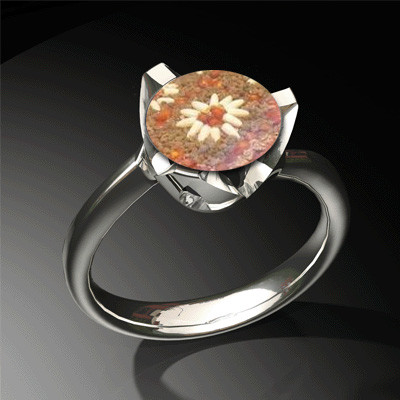
\includegraphics[scale=.66]{figures/annexes/qiegao/2.jpg}}
    \caption{
      Qiegao
    }
\end{figure}

\clearpage
\subsection{The Voice of China}

\url{http://en.wikipedia.org/wiki/The_Voice_of_China}

\begin{figure}[h!]
    \centering
    \subfloat[Logo Officiel de The Voice of China]{
\includegraphics[scale=.47]{figures/annexes/thevoice/The_Voice_of_China_-_official_logo.jpg}}
    \subfloat[Les membres du Jury de l'édition 2014]{
\includegraphics[scale=.5]{figures/annexes/thevoice/The_Voice_of_China_S2.jpg}}
    \newline
    \subfloat[``The Voice devient le sujet le plus discuté du mois de Juillet'', d'après Hi News, \url{http://www.hinews.cn/news/system/2012/08/25/014863154.shtml}, consulté le 7 Juillet à 14:32]{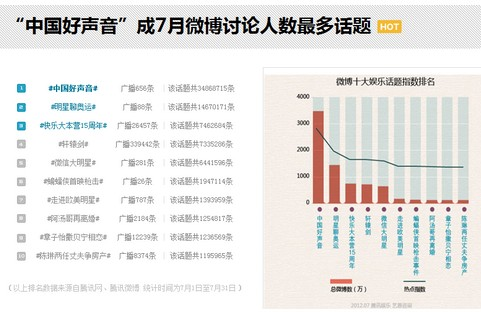
\includegraphics[scale=.8]{figures/annexes/thevoice/weibo-trends.jpg}}
    \subfloat[Un dessin posté par un utilisateur de Sina Weibo]{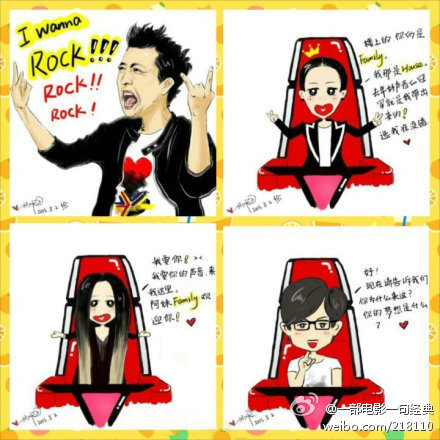
\includegraphics[scale=.42]{figures/annexes/thevoice/7ff5fbaftw1e7ilgxti2bj20c80c8gn2.jpg}}
    \caption{
      The Voice of China : Illustrations
    }
\end{figure}


% \clearpage
% \subsection{Moyan}

% \url{http://en.wikipedia.org/wiki/Mo_Yan}

% \begin{figure}[h!]
%     \centering
%     \subfloat[Logo Officiel de The Voice of China]{
\includegraphics[scale=.47]{figures/annexes/thevoice/The_Voice_of_China_-_official_logo.jpg}}
%     \subfloat[Les membres du Jury de l'édition 2014]{
\includegraphics[scale=.5]{figures/annexes/thevoice/The_Voice_of_China_S2.jpg}}
%     \newline
%     \subfloat[``The Voice devient le sujet le plus discuté du mois de Juillet'', d'après Hi News, \url{http://www.hinews.cn/news/system/2012/08/25/014863154.shtml}, consulté le 7 Juillet à 14:32]{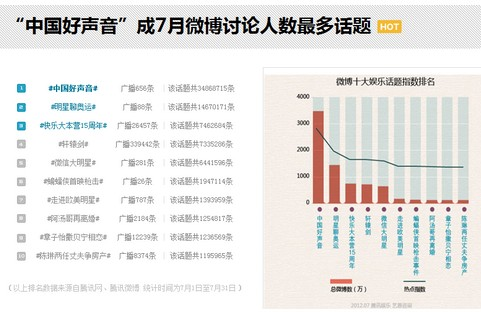
\includegraphics[scale=.8]{figures/annexes/thevoice/weibo-trends.jpg}}
%     \subfloat[Un dessin posté par un utilisateur de Sina Weibo]{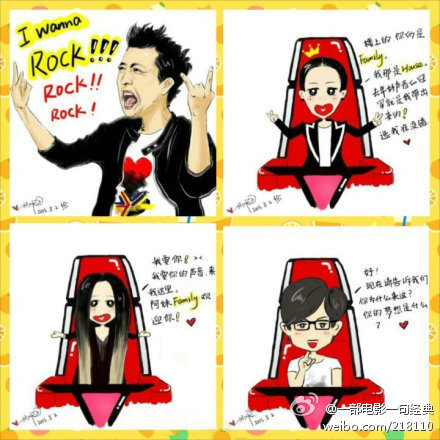
\includegraphics[scale=.42]{figures/annexes/thevoice/7ff5fbaftw1e7ilgxti2bj20c80c8gn2.jpg}}
%     \caption{
%       The Voice of China : Illustrations
%     }
% \end{figure}
